\documentclass[12pt]{iopart}
\usepackage{graphicx}% Include figure files

\bibliographystyle{PV}
\begin{document}
\title[]{Acoustically driven degradation in single crystalline Si solar cell}

\author{O Ya Olikh}

\address{Faculty of Physics, Taras Shevchenko National University of Kyiv, Kyiv 01601, Ukraine}
\ead{olikh@univ.kiev.ua}

\begin{abstract}
Abstract Abstract Abstract Abstract Abstract Abstract Abstract Abstract Abstract Abstract
Abstract Abstract Abstract Abstract Abstract Abstract Abstract Abstract Abstract Abstract
Abstract Abstract Abstract Abstract Abstract Abstract Abstract Abstract Abstract Abstract
Abstract Abstract Abstract Abstract Abstract Abstract Abstract Abstract Abstract Abstract
Abstract Abstract Abstract Abstract Abstract Abstract Abstract Abstract Abstract Abstract
Abstract Abstract Abstract Abstract Abstract Abstract Abstract Abstract Abstract Abstract
Abstract Abstract Abstract Abstract Abstract Abstract Abstract Abstract Abstract Abstract
Abstract Abstract Abstract Abstract Abstract Abstract Abstract Abstract Abstract Abstract
Abstract Abstract Abstract Abstract Abstract Abstract Abstract Abstract Abstract Abstract
\end{abstract}

%\pacs{73.30.+y, 43.35.Ty, 43.35.+d, 72.20.-i, 73.40.-c}
\noindent{Keywords: \it silicon, solar cells, ultrasound influence\/ }

%\maketitle

%\ioptwocol


\section{Introduction}

The silicon solar cells (SSC) are still dominant in the photovoltaic (PV) field due to their high efficiency, low selling price and process maturity.
Therefore, understanding the way of material properties modification is a top priority for  most of PV device manufacturers.
It is known, for example, the loss in the SSC efficiency is observed in consequence of
excess carrier injection by above-bandgap illumination or forward biasing \cite{LID:BothePP,LID:SchmidtJMR,LIDRev} (so-called light-induced degradation or LID),
high voltage stress \cite{PID:SEMSC,PID:PP} (potential-induced degradation or PID),
or radiation treatment \cite{Bhat,Karazhanov} (irradiation-induced degradation or IID).
Degradation reasons are processes in crystal defect sub-system under external influence.
It is may be a transformation of the boron-oxygen or copper-contained complex (for the LID case),
a decoration of stacking faults by sodium (PID case) or
a creation of radiation-induced recombination centers (IID case).
The partial or full SSC efficiency recovery is observed quite often during of subsequent annealing at an elevated temperature.

On the other hand, it has been shown experimentally that ultrasonic  waves (USWs) can be the effective instrument for defect engineering in silicon.
In particular, ultrasound is used
to affect a carrier diffusion length \cite{Ostapenko1999,Ostrovskii2001},
to vary a current in  p--n structures and Schottky diodes \cite{OlikhJAP,Olikh2011Sem,Davletova2009,Davletova2008,YOlikh2005,Olikh:Ultras},
to transform an impurity defect \cite{Korotchenkov1995,Ostapenko1995,Olikh2009Sem},
to change a spectrum  \cite{Zaver:2008} and density \cite{Mirsagatov} of surface states.
Frequently the crystal and device properties recover after stopping of ultrasound action at room temperature even \cite{Ostapenko1999,Ostrovskii2001,OlikhJAP,Korotchenkov1995}.

This article presents the result of experimentally investigation of the acoustic strain field influence on the electrical characteristic of the n$^+$--p SSC.
Ultrasound has been found to result the decrease of carriers lifetime and, accordingly, solar cell efficiency.
The USWs intensity did not exceed $0.5$~W/cm$^2$ and the full recovery of cell characteristics was observed.
Dependencies of such sound induced degradation on USW type and intensity are presented.
%Features of such sound induced degradation are presented.
The findings are discussed by using model of coupled defect level recombination \cite{CDLR:JAP,CDLR:JAP1995}.



\section{Experimental and calculation details}

The investigated solar cell was created on 2 inch p-type CZ-Si:B wafers with doping level of $1.4\times10^{15}$~cm$^{-3}$ and thickness of 300~$\mu$m.
The n$^+$--layer with carrier concentration of about $10^{19}$~cm$^{-3}$ and thickness of 0.5~$\mu$m was created by phosphorus implantation.
Then wafer surface were passivated by Al$_2$O$_3$ film and further capped by TiO$_x$ as antireflective coating.
Finally the aluminium solid contact and metal grid was fabricated on p-- and n--surface respectively.
The samples with area of $1.5$ to $2.1$~cm$^{2}$ used in our experiments were cut from the central part of the wafer.

The dark and illuminated forward current-voltage ($I$--$V$) characteristics of the samples were measured over a temperature range 290--340~K.
The sample temperature was controlled by differential copper-constantan thermocouple.
Some curves are shown in \Fref{figIV}.
The classical double-diode model of SSC $I$--$V$ characteristics expressed in the following form:
\begin{eqnarray}
\label{eqIV}
\nonumber I(V,T)&=&-I_{ph}+I_{01}\left\{\exp \left[\frac{q(V-IR_s)}{kT}\right]-1\right\}\\ 
&&+I_{0n}\left\{\exp \left[\frac{q(V-IR_s)}{nkT}\right]-1\right\}+\frac{V-IR_s}{R_{sh}}\,,
\end{eqnarray}
where $I_{01}$ and $I_{0n}$ are the saturation current densities of the ideal and nonideal components, 
$n$ is the ideality factor of the nonideal current components, 
$R_s$ and $R_{sh}$ are the series and shunt resistances of the device,
$I_{ph}$ is the photocurrent. 
The current-voltage  equation that models the solar cell by  an equivalent electrical circuit contains several parameters related to physical phenomena occurring in  the device.
It is commonly believed that $I_{01}$ is closely related to recombination in the quasi-neutral region and in an n$^+$--p diode can be written as follows:
\begin{equation}
\label{eqI01}
    I_{01}=\frac{qAn_i^2}{N_A}\sqrt{\frac{\mu_nkT}{\tau_n}}\,,
\end{equation}
where $A$ is the cell area,
$n_i$ is the intrinsic carrier concentration,
$N_A$ is the doping density in the $p$ region,
$\mu_n$ and $\tau_n$ are the electron (minority carrier) mobility and lifetime outside space charge region (SCR).
$I_{0n}$ reflects the overall recombination in the SCR and may be expressed as
\begin{equation}
\label{eqI0n}
    I_{0n}=\frac{qAWn_i}{2\tau_{g}}\,,
\end{equation}
where $\tau_{g}$ is the carrier lifetime in the SCR,
$W$ is the SCR thickness:
\begin{equation}
\label{eqW}
    W(V,T)=\sqrt{\frac{2 \varepsilon \varepsilon_0(N_A+N_D)}{q N_A N_D}\left[\frac{E_g}{q}-\frac{kT}{q}\ln\left(\frac{N_vN_c}{N_AN_D}\right)-\frac{2kT}{q}-V\right]} \,,
\end{equation}
$\varepsilon$ is the permittivity (11.7 for Si),
$N_D$ is the doping density in the $n$ region,
$E_g$ is the semiconductor band gap,
$N_c$ and $N_v$ are the the effective density of states in the conduction and valence bands.




\begin{figure}
\begin{center}
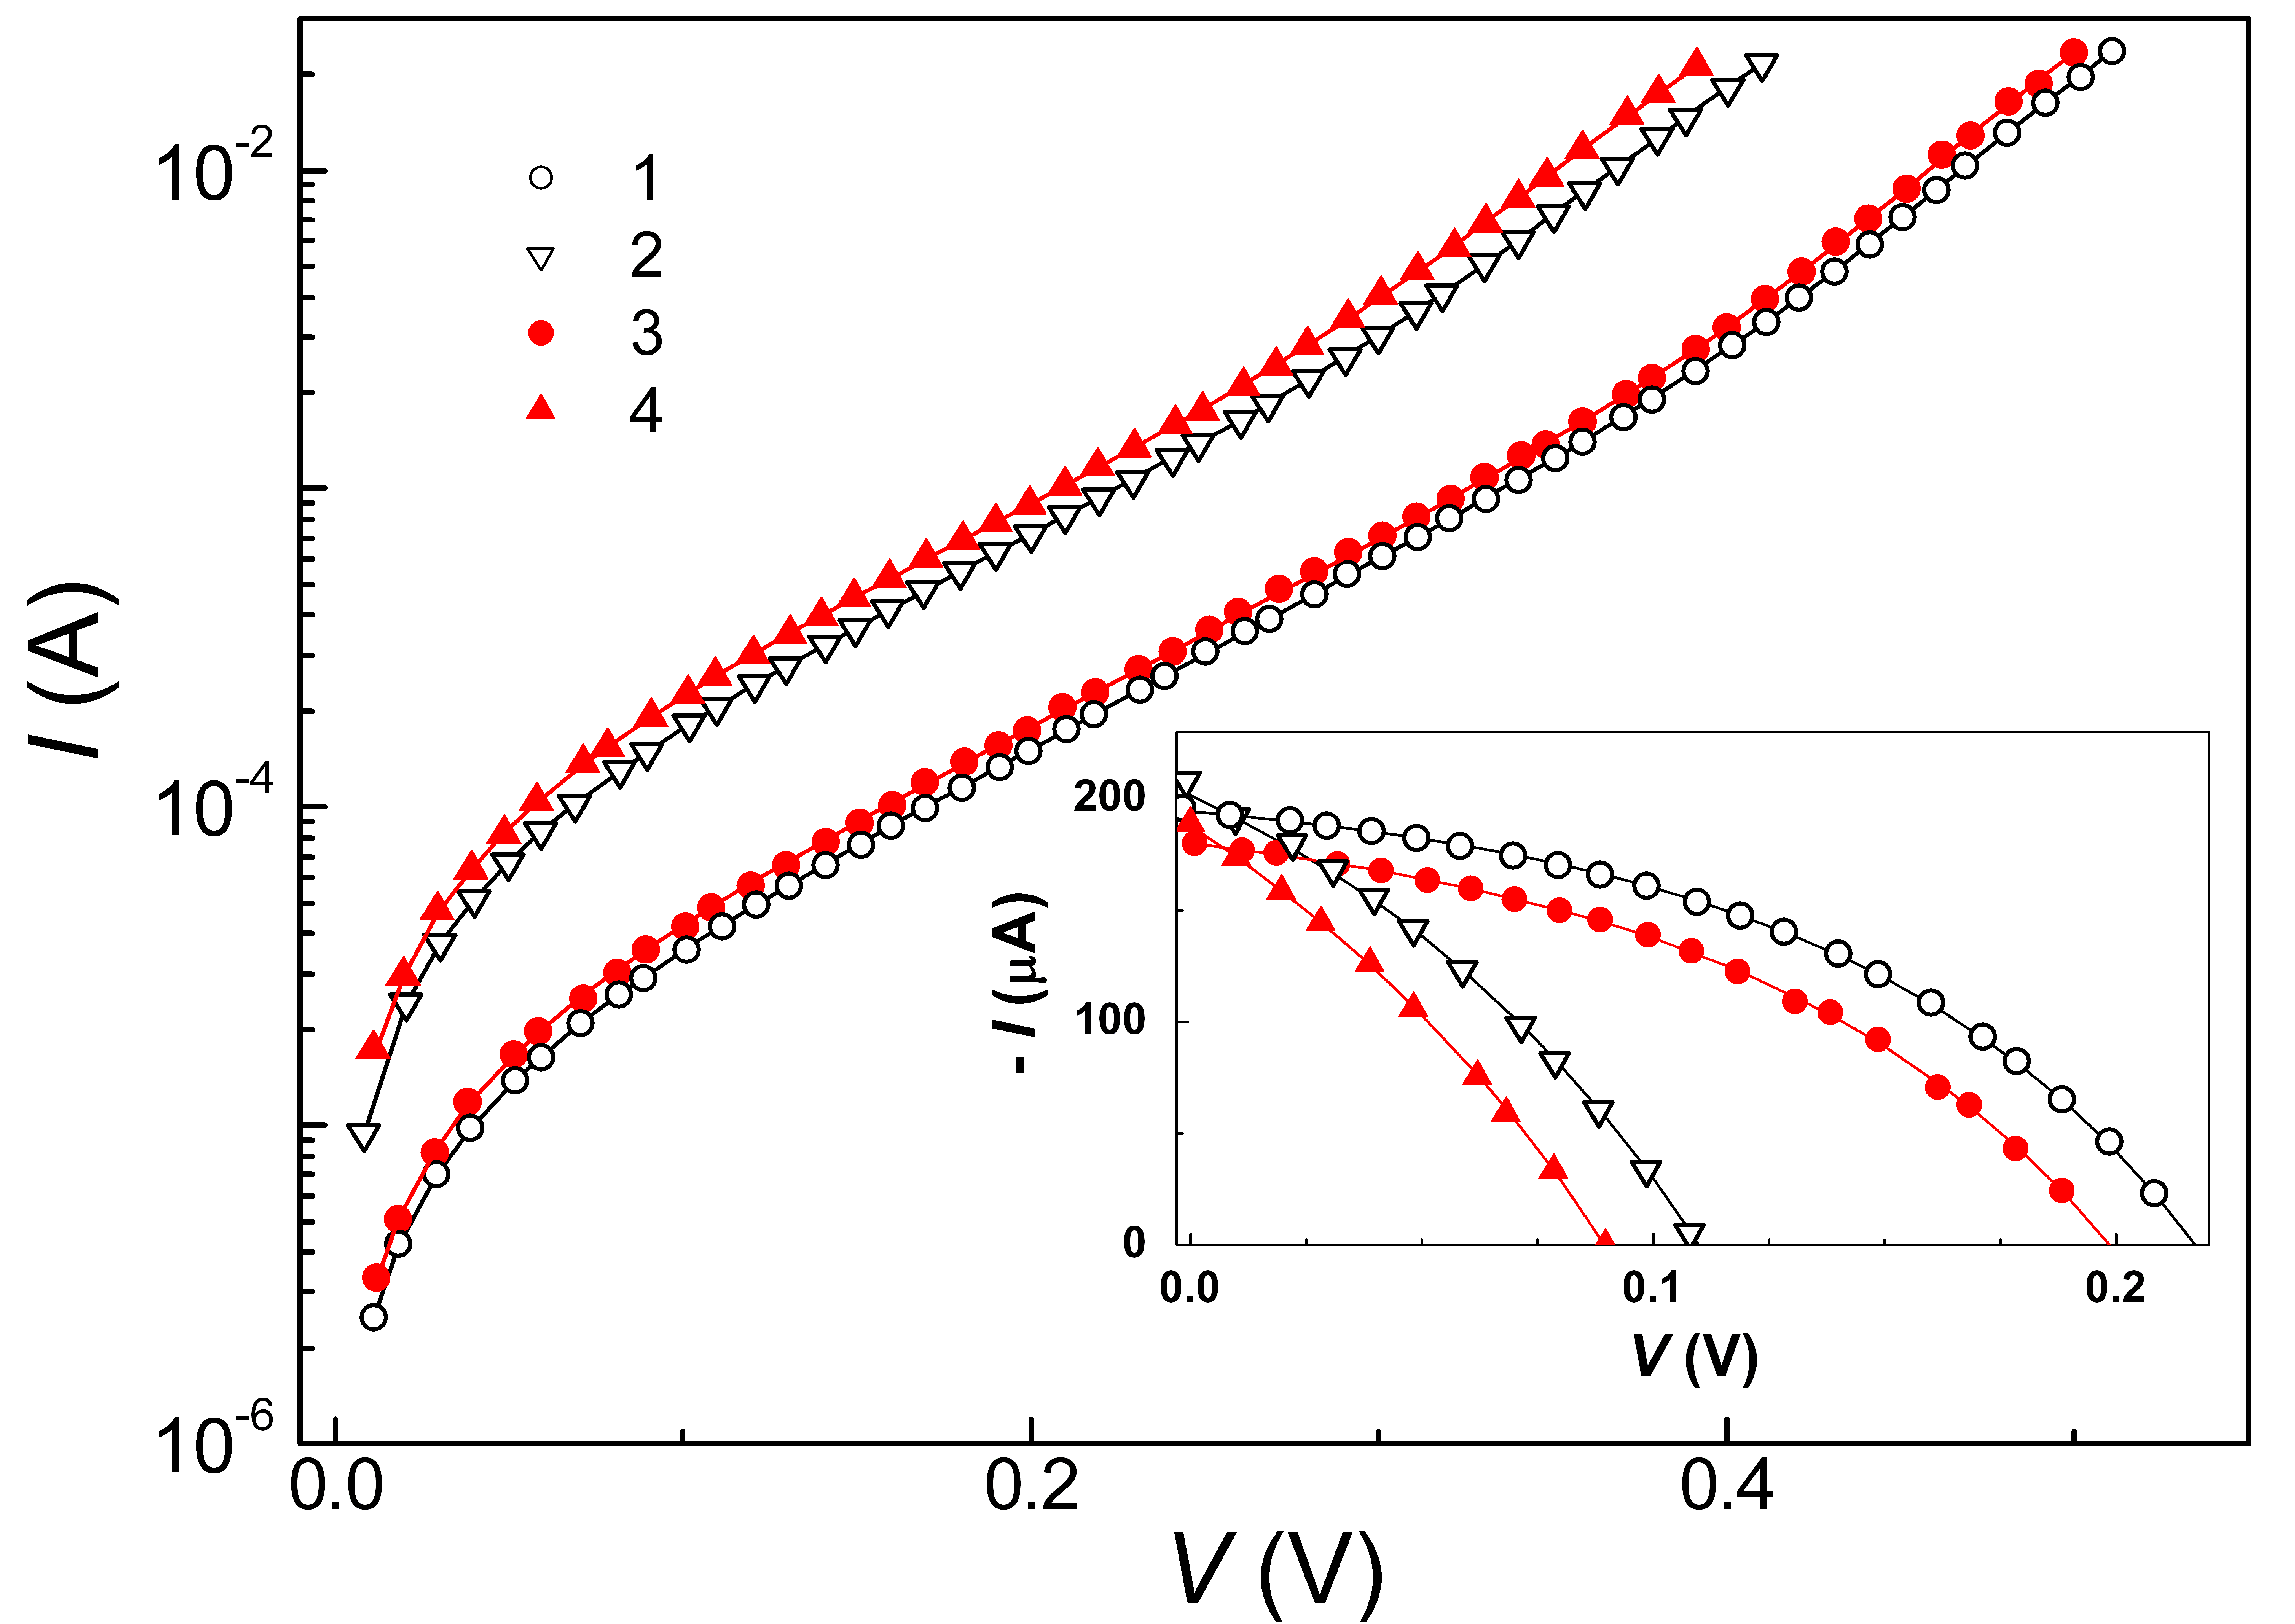
\includegraphics[width=7.5cm]{olikhFig1}%
\end{center}
\caption{\label{figIV}
SSC dark $I$--$V$ characteristics measured at 301~K (curves 1, 3) and 341~K (curves 2, 4)
with (2, 4) and without(1, 3) USL.
$W_{U\!S}^T=0.40$~W/cm$^2$.
Inset: Parts of illuminated $I$--$V$ characteristics in the voltage range from 0 to $V_{oc}$.
Lines are the fitted curves using Eq. (1).
}%
\end{figure}


The revers current-voltage ($I$--$V$) characteristics of the samples both with and without US loading were measured in the temperature range from 130 to 330~K.
In case of US loading, the longitudinal waves excited in the samples were $4.1$ and $8.4$~MHz in frequency $f_{U\!S}$ and had the intensity of $W_{U\!S} < 0.8$~ W/cm$^2$.
It was reported previously \cite{Ostapenko1995,Olikh:Ultras,Olikh2011Sem,Ostrovskii2001} that a characteristic time of change in the silicon structure parameters under the ultrasound action  did not exceed $2\cdot10^3$~s.
In order to wait till the acoustically induced transitional period the following experimental procedure was used.
After USL start the sample was kept at room temperature during 30 min.
Then the sample was cooled to 130~K.
The cooling time was about a half of hour.
After cooling the $I$--$V$ measurements and the sample heating were started.
The sample temperature was controlled by differential copper-constantan thermocouple.

In order to avoid the effect of piezoelectric field on $I$--$V$ characteristics, the piezoelectric cell was shielded and aluminium acoustic line was used.
The more details about the experimental setup are presented elsewhere \cite{OlikhJAP}.

The data non-linear fitting were done by using the differential evolution method \cite{DEWang}.

\section{Results and Discussion}
\subsection{Ultrasound influence on reverse current}


\Fref{figIVT} shows the complete $I$-�$V$-�$T$ characteristics that were measured without US loading.
To avoid a busy looking graph, the selection of measured $I$--$V$ characteristics is shown in this figure.
Below the reverse branches only are under consideration .
It is  a universal observation that the current from any SD never truly saturates at large reverse bias.
Such "soft" reverse characteristics are observed for structures under investigation too.
One can see that the reverse current change with the bias increase is larger at the low temperature.




Therefore $I_1$ can be described as follows
\begin{equation}\label{eqIte}
    I_1=I_0T^2\exp(-q\Phi_b/kT)[1-\exp(-V_R/kT)]\,,
\end{equation}
where $\Phi_b$ is zero bias Schottky barrier height (SBH),
$I_0$ is the constant.
It is predicted theoretically \cite{Rhoderick1988} and observed
experimentally \cite{Aboelfotoh,Zhua}, that the SBH decreases with temperature increase in the way similar to semiconductor band gap.


\section{Conclusion}
The experimental investigation of ultrasound influence on the reverse leakage current of Mo/$n$-$n^{+}$-Si Schottky barrier structure has been carried out in the temperature range from 130 to 330~K.
The investigation has revealed the acoustically induced reversible increase of reverse current.
The efficiency of ultrasound influence decreases with the bias and the temperature rising and increases with the acoustic waves frequency growth.
The analysis has shown that the thermionic emission and the phonon-assisted tunneling make a major contribution to the leakage current and both mechanisms are affected by ultrasound.
It has been found that the ultrasonic loading leads to the decrease of barrier height, trap depth, occupied interface state density, Poole--Frenkel factor.
Thus, ultrasound can be an effective tool for controlling metal�-semiconductor structure characteristics.

\section*{References}
%\bibliographystyle{JoS}
\bibliography{olikh}

\end{document}

